% Options for packages loaded elsewhere
\PassOptionsToPackage{unicode}{hyperref}
\PassOptionsToPackage{hyphens}{url}
%
\documentclass[
  doc]{apa6}
\usepackage{amsmath,amssymb}
\usepackage{iftex}
\ifPDFTeX
  \usepackage[T1]{fontenc}
  \usepackage[utf8]{inputenc}
  \usepackage{textcomp} % provide euro and other symbols
\else % if luatex or xetex
  \usepackage{unicode-math} % this also loads fontspec
  \defaultfontfeatures{Scale=MatchLowercase}
  \defaultfontfeatures[\rmfamily]{Ligatures=TeX,Scale=1}
\fi
\usepackage{lmodern}
\ifPDFTeX\else
  % xetex/luatex font selection
\fi
% Use upquote if available, for straight quotes in verbatim environments
\IfFileExists{upquote.sty}{\usepackage{upquote}}{}
\IfFileExists{microtype.sty}{% use microtype if available
  \usepackage[]{microtype}
  \UseMicrotypeSet[protrusion]{basicmath} % disable protrusion for tt fonts
}{}
\makeatletter
\@ifundefined{KOMAClassName}{% if non-KOMA class
  \IfFileExists{parskip.sty}{%
    \usepackage{parskip}
  }{% else
    \setlength{\parindent}{0pt}
    \setlength{\parskip}{6pt plus 2pt minus 1pt}}
}{% if KOMA class
  \KOMAoptions{parskip=half}}
\makeatother
\usepackage{xcolor}
\usepackage{graphicx}
\makeatletter
\def\maxwidth{\ifdim\Gin@nat@width>\linewidth\linewidth\else\Gin@nat@width\fi}
\def\maxheight{\ifdim\Gin@nat@height>\textheight\textheight\else\Gin@nat@height\fi}
\makeatother
% Scale images if necessary, so that they will not overflow the page
% margins by default, and it is still possible to overwrite the defaults
% using explicit options in \includegraphics[width, height, ...]{}
\setkeys{Gin}{width=\maxwidth,height=\maxheight,keepaspectratio}
% Set default figure placement to htbp
\makeatletter
\def\fps@figure{htbp}
\makeatother
\setlength{\emergencystretch}{3em} % prevent overfull lines
\providecommand{\tightlist}{%
  \setlength{\itemsep}{0pt}\setlength{\parskip}{0pt}}
\setcounter{secnumdepth}{-\maxdimen} % remove section numbering
% Make \paragraph and \subparagraph free-standing
\makeatletter
\ifx\paragraph\undefined\else
  \let\oldparagraph\paragraph
  \renewcommand{\paragraph}{
    \@ifstar
      \xxxParagraphStar
      \xxxParagraphNoStar
  }
  \newcommand{\xxxParagraphStar}[1]{\oldparagraph*{#1}\mbox{}}
  \newcommand{\xxxParagraphNoStar}[1]{\oldparagraph{#1}\mbox{}}
\fi
\ifx\subparagraph\undefined\else
  \let\oldsubparagraph\subparagraph
  \renewcommand{\subparagraph}{
    \@ifstar
      \xxxSubParagraphStar
      \xxxSubParagraphNoStar
  }
  \newcommand{\xxxSubParagraphStar}[1]{\oldsubparagraph*{#1}\mbox{}}
  \newcommand{\xxxSubParagraphNoStar}[1]{\oldsubparagraph{#1}\mbox{}}
\fi
\makeatother
% definitions for citeproc citations
\NewDocumentCommand\citeproctext{}{}
\NewDocumentCommand\citeproc{mm}{%
  \begingroup\def\citeproctext{#2}\cite{#1}\endgroup}
\makeatletter
 % allow citations to break across lines
 \let\@cite@ofmt\@firstofone
 % avoid brackets around text for \cite:
 \def\@biblabel#1{}
 \def\@cite#1#2{{#1\if@tempswa , #2\fi}}
\makeatother
\newlength{\cslhangindent}
\setlength{\cslhangindent}{1.5em}
\newlength{\csllabelwidth}
\setlength{\csllabelwidth}{3em}
\newenvironment{CSLReferences}[2] % #1 hanging-indent, #2 entry-spacing
 {\begin{list}{}{%
  \setlength{\itemindent}{0pt}
  \setlength{\leftmargin}{0pt}
  \setlength{\parsep}{0pt}
  % turn on hanging indent if param 1 is 1
  \ifodd #1
   \setlength{\leftmargin}{\cslhangindent}
   \setlength{\itemindent}{-1\cslhangindent}
  \fi
  % set entry spacing
  \setlength{\itemsep}{#2\baselineskip}}}
 {\end{list}}
\usepackage{calc}
\newcommand{\CSLBlock}[1]{\hfill\break\parbox[t]{\linewidth}{\strut\ignorespaces#1\strut}}
\newcommand{\CSLLeftMargin}[1]{\parbox[t]{\csllabelwidth}{\strut#1\strut}}
\newcommand{\CSLRightInline}[1]{\parbox[t]{\linewidth - \csllabelwidth}{\strut#1\strut}}
\newcommand{\CSLIndent}[1]{\hspace{\cslhangindent}#1}
\ifLuaTeX
\usepackage[bidi=basic]{babel}
\else
\usepackage[bidi=default]{babel}
\fi
\babelprovide[main,import]{english}
% get rid of language-specific shorthands (see #6817):
\let\LanguageShortHands\languageshorthands
\def\languageshorthands#1{}
% Manuscript styling
\usepackage{upgreek}
\captionsetup{font=singlespacing,justification=justified}

% Table formatting
\usepackage{longtable}
\usepackage{lscape}
% \usepackage[counterclockwise]{rotating}   % Landscape page setup for large tables
\usepackage{multirow}		% Table styling
\usepackage{tabularx}		% Control Column width
\usepackage[flushleft]{threeparttable}	% Allows for three part tables with a specified notes section
\usepackage{threeparttablex}            % Lets threeparttable work with longtable

% Create new environments so endfloat can handle them
% \newenvironment{ltable}
%   {\begin{landscape}\centering\begin{threeparttable}}
%   {\end{threeparttable}\end{landscape}}
\newenvironment{lltable}{\begin{landscape}\centering\begin{ThreePartTable}}{\end{ThreePartTable}\end{landscape}}

% Enables adjusting longtable caption width to table width
% Solution found at http://golatex.de/longtable-mit-caption-so-breit-wie-die-tabelle-t15767.html
\makeatletter
\newcommand\LastLTentrywidth{1em}
\newlength\longtablewidth
\setlength{\longtablewidth}{1in}
\newcommand{\getlongtablewidth}{\begingroup \ifcsname LT@\roman{LT@tables}\endcsname \global\longtablewidth=0pt \renewcommand{\LT@entry}[2]{\global\advance\longtablewidth by ##2\relax\gdef\LastLTentrywidth{##2}}\@nameuse{LT@\roman{LT@tables}} \fi \endgroup}

% \setlength{\parindent}{0.5in}
% \setlength{\parskip}{0pt plus 0pt minus 0pt}

% Overwrite redefinition of paragraph and subparagraph by the default LaTeX template
% See https://github.com/crsh/papaja/issues/292
\makeatletter
\renewcommand{\paragraph}{\@startsection{paragraph}{4}{\parindent}%
  {0\baselineskip \@plus 0.2ex \@minus 0.2ex}%
  {-1em}%
  {\normalfont\normalsize\bfseries\itshape\typesectitle}}

\renewcommand{\subparagraph}[1]{\@startsection{subparagraph}{5}{1em}%
  {0\baselineskip \@plus 0.2ex \@minus 0.2ex}%
  {-\z@\relax}%
  {\normalfont\normalsize\itshape\hspace{\parindent}{#1}\textit{\addperi}}{\relax}}
\makeatother

\makeatletter
\usepackage{etoolbox}
\patchcmd{\maketitle}
  {\section{\normalfont\normalsize\abstractname}}
  {\section*{\normalfont\normalsize\abstractname}}
  {}{\typeout{Failed to patch abstract.}}
\patchcmd{\maketitle}
  {\section{\protect\normalfont{\@title}}}
  {\section*{\protect\normalfont{\@title}}}
  {}{\typeout{Failed to patch title.}}
\makeatother

\usepackage{xpatch}
\makeatletter
\xapptocmd\appendix
  {\xapptocmd\section
    {\addcontentsline{toc}{section}{\appendixname\ifoneappendix\else~\theappendix\fi: #1}}
    {}{\InnerPatchFailed}%
  }
{}{\PatchFailed}
\makeatother
\keywords{EEG, Eye State Classification, Machine Learning, Logistic Regression, LASSO Feature Selection, Random Forest, SVM, MLP, kNN\newline\indent Word count: 3,015}
\usepackage{csquotes}
\usepackage{float}
\usepackage[justification=centering]{caption}
\usepackage{fancyhdr}
\pagestyle{fancy}
\fancyhead[LO]{}
\ifLuaTeX
  \usepackage{selnolig}  % disable illegal ligatures
\fi
\usepackage{bookmark}
\IfFileExists{xurl.sty}{\usepackage{xurl}}{} % add URL line breaks if available
\urlstyle{same}
\hypersetup{
  pdftitle={EEG Eye State Classification Using Machine Learning Techniques},
  pdfauthor={Chun-Chien Hsueh1},
  pdflang={en-EN},
  pdfkeywords={EEG, Eye State Classification, Machine Learning, Logistic Regression, LASSO Feature Selection, Random Forest, SVM, MLP, kNN},
  hidelinks,
  pdfcreator={LaTeX via pandoc}}

\title{EEG Eye State Classification Using Machine Learning Techniques}
\author{Chun-Chien Hsueh\textsuperscript{1}}
\date{}


\shorttitle{SHORT TITLE}

\authornote{

Correspondence concerning this article should be addressed to Chun-Chien Hsueh. E-mail: \href{mailto:ch1236@scarletmail.rutgers.edu}{\nolinkurl{ch1236@scarletmail.rutgers.edu}}

}

\affiliation{\vspace{0.5cm}\textsuperscript{1} Department of Statistics, Rutgers University}

\abstract{%
Brain-computer interface (BCI) technology enables human-computer interaction by measuring brain electrical activity and is widely used in the fields of medicine and neuroscience. EEG signals are used to monitor brain states, such as detecting fatigue or attention, due to their non-invasive nature, but high noise and data imbalance often limit their classification accuracy. This study explored the use of EEG data for eye state (eyes open or closed) classification. We processed the EEG eye state dataset from the UCI Machine Learning Repository using oversampling, the least absolute shrinkage and selection operator (LASSO), and random forest feature selection. Five machine learning models were used for modeling -- random forest, logistic regression, support vector machine (SVM), multi-layer perceptron (MLP), and k-nearest neighbor (kNN), among which SVM achieved the highest test accuracy (0.946) and AUC value (0.982). The McNemar test showed that logistic regression performed significantly worse (p \textless{} 0.001), while SVM, MLP, and kNN performed similarly (p \textgreater{} 0.05). The learning curve analysis shows that SVM has robust generalization ability, but random forest has a tendency to overfit. Feature analysis highlights the physiological importance of time domain (window\_start) and frequency domain features (e.g., fft\_beta\_power\_p8). This study demonstrates the effectiveness of advanced feature engineering and machine learning in EEG classification.
}



\begin{document}
\maketitle

\newpage

\section{I. Introduction}\label{i.-introduction}

Electroencephalogram (EEG) is a non-invasive brain activity monitoring technology that uses an electroencephalogram to record the activity of electrical currents generated by brain cells on the surface of the brain. EEG signals can capture tiny changes in the brain's electrical activity. The brain waves that represent the state of the brain can generally be divided into five types: Alpha, Beta, Theta, Delta, Gamma, each of which has different strengths in different activities. It is easy to implement and widely used in medical diagnosis, neuroengineering, biomedical engineering (brain-computer interface (BCI), sleep analysis, and epilepsy detection), etc. In particular, eye status (eyes open or closed) is of great significance in research such as driving fatigue monitoring, attention assessment, and medical auxiliary diagnosis. Automatically identifying eye states by analyzing EEG signal data can effectively help solve the research problems mentioned above. However, since the intensity of brain waves is only a few hundred microvolts, they are easily distorted by external interference or noise (high noise). As a result, it is a huge challenge to improve classification performance through reliable data processing and the use of advanced modeling methods.
This study focuses on using machine learning technology to improve the accuracy and stability of eye state prediction. Specifically, the EEG eye state dataset in the UCI machine learning library is used to perform data preprocessing such as standardization, noise reduction, and feature engineering to generate a feature set. The oversampling technique is used to solve the data imbalance problem, and then LASSO and random forest are used for feature selection to screen out the features that contribute most to the prediction and eliminate potential collinearity. Finally, Logistic regression, SVM, MLP, kNN models were trained and their performance was compared using accuracy, ROC curve, AUC, and McNemar test. The remainder of the paper is organized as follows: Section II reviews the relevant literature, Section III introduces the data and methods, Section IV presents the results and discussion, and finally Section V summarizes the research findings and looks forward to future work.

\section{II. Literature Review}\label{ii.-literature-review}

Eye state classification, as a classic task of EEG analysis, has been widely used as material for analysis research. Early studies mainly focused on manual feature extraction and simple classifiers. For example, Roesler and Suendermann (2013) proposed a prediction method for EEG data based on incremental attribute learning, demonstrating the role of feature selection in improving prediction performance. However, such methods have hard to capture complex patterns of signals and are difficult to adapt to the needs of large-scale datasets containing a large number of features. With the development of machine learning technology, the performance of EEG eye state classification has been significantly improved. Support vector machine (SVM) has become a commonly used method due to its classification ability and generalization performance in high-dimensional space. Singla, Singh, and Jha (2011) compared the performance of SVM and artificial neural network (ANN) in EEG eye state (blinking, eyes closed, eyes open) detection and found that SVM performed better than ANN in terms of stability and accuracy. Multilayer Perceptron (MLP) is a deep neural network that can effectively capture complex patterns in EEG signals through multiple layers of nonlinear processing. Sabanci and Koklu (2015) used the EEG eye state data from the UCI machine learning library and modeled it using k-nearest neighbor (kNN) and MLP models. Their results showed good performance of kNN, achieving an accuracy of about 84\% under the best configuration.

In EEG eye state classification, interactive features, such as the electrode differences between the left and right brain, can help improve the classification effect. Ma and Gao (2020) proposed a model that combines factorization machine (FM) and long short-term memory network (LSTM), emphasizing the importance of feature interaction for eye behavior prediction. Wang, Chen, and Zhang (2014) used the incremental attribute learning (IAL) method to gradually introduce features to reduce interference and improve classification performance, showing the importance of feature selection and interaction.

\section{III. Data and Methods}\label{iii.-data-and-methods}

\subsection{3.1 Data description}\label{data-description}

The UCI Machine Learning Repository (2013) dataset is used in this study, trying to \textbf{predict eye states (open or closed)}. This dataset was recored from a 28 year-old healthy man, contains 14,980 instance of EEG reading collected by Emotiv EEG headset. Each instance includes 14 continuous EEG features representing voltage measurements (in microvolts) and a binary target variable, \textbf{eyeDetection}, indicating the eye state (0 for eyes closed, 1 for eyes open). The data was recorded at a sampling rate of 128 Hz, with about 117 seconds record period. \textbf{Table 1} indicates the brain regions represented by each channel.

\begin{table}[!h]
\centering
\caption{\label{tab:electrode-table}EEG Electrode Locations and Corresponding Brain Regions}
\centering
\begin{tabular}[t]{l|l}
\hline
Electrode & Brain.Region\\
\hline
AF3 & Left prefrontal cortex\\
\hline
F7 & Left frontal lobe\\
\hline
F3 & Left frontal cortex\\
\hline
FC5 & Left frontocentral area\\
\hline
T7 & Left temporal lobe\\
\hline
P7 & Left parietal lobe\\
\hline
O1 & Left occipital lobe\\
\hline
O2 & Right occipital lobe\\
\hline
P8 & Right parietal lobe\\
\hline
T8 & Right temporal lobe\\
\hline
FC6 & Right frontocentral area\\
\hline
F4 & Right frontal cortex\\
\hline
F8 & Right frontal lobe\\
\hline
AF4 & Right prefrontal cortex\\
\hline
\end{tabular}
\end{table}

\newpage

\subsection{3.2 Data pre-processing}\label{data-pre-processing}

\begin{itemize}
\tightlist
\item
  \textbf{Tidy data}: Make sure the data is tidy and eyeDetection is factor. Checking there is no missing value.
\item
  \textbf{Standardization}: EEG signals were standardized using the \texttt{scale()} function to ensure zero mean and unit variance across all features, mitigating the impact of scale differences.
\item
  \textbf{Denoising}: A moving average filter with a window size of 5 was applied to smooth the data and reduce high-frequency noise, preserving the underlying signal trends.
\end{itemize}

\subsection{3.3 Feature engineering}\label{feature-engineering}

\begin{itemize}
\item
  \textbf{Frequency features}: Power spectral density was extracted using Fast Fourier Transform (FFT) across five frequency bands: \texttt{Delta} (0.5--4 Hz), \texttt{Theta} (4--8 Hz), \texttt{Alpha} (8--13 Hz), \texttt{Beta} (13--30 Hz), and \texttt{Gamma} (30--50 Hz). These features capture the brain's rhythmic activity associated with different states.
\item
  \textbf{Interaction features}: Biologically meaningful features such as AF\_diff (AF3 - AF4), O\_diff (O1 - O2), AF3\_O1\_interaction (AF3 × O1), alpha\_O1\_alpha\_AF3\_diff (fft\_alpha\_power\_O1 - fft\_alpha\_power\_AF3), and beta\_alpha\_ratio\_FC5 (fft\_beta\_power\_FC5 / fft\_alpha\_power\_FC5) were selectively included. The selection of these features is based on knowledge in the field of EEG. AF3 and AF4 are located in the prefrontal lobe and are closely related to attention-related cognitive activities. Their difference can reflect the asymmetry of the left and right brain, which may be indicative of eye states (such as eyes closed and eyes open); O1 and O2 are located in the occipital lobe and are responsible for visual processing. Their difference can capture the spatial differences in the visual cortex; the interaction term between AF3 and O1 takes into account the functional connection between the prefrontal and occipital lobes, which may be related to visual attention regulation; the difference and ratio of Alpha and Beta band power (such as alpha\_O1\_alpha\_AF3\_diff and beta\_alpha\_ratio\_FC5) reflect the activity differences of different brain regions in relaxation (Alpha band, 8--13 Hz) and alertness (Beta band, 13--30 Hz) states.
\item
  \textbf{Statistical features}: Skewness and kurtosis were computed for each channel within sliding windows to capture the shape and distribution of the EEG signals.
\item
  \textbf{Oversampling}: To address the class imbalance problem in the dataset, oversampling technique was applied using the \texttt{upSample()} function. This method ensures that the minority class is fully represented during training by randomly replicating the minority class (closed eyes) samples to make the number of samples in the two classes equal.
\end{itemize}

\subsection{3.4 Feature selecton}\label{feature-selecton}

To reduce the data dimension and eliminate collinearity, the following feature selection techniques were performed:

\begin{itemize}
\item
  \textbf{LASSO}: Using \texttt{cv.glmnet} function to perform least absolute shrinkage and selection operator(LASSO). LASSO reduces the coefficients of unimportant features to zero through L1 regularization, thereby selecting important predictors. The optimal lambda.1se is selected through ten-fold cross validation to balance model complexity and performance.
\item
  \textbf{Random Forest}: After feature selection by LASSO, a random forest model was trained. Feature importance was ranked based on the \texttt{MeanDecreaseGini} metric and the top 30 features were selected for subsequent modeling, ensuring that only the most predictive features were chosen.
\end{itemize}

\subsection{3.5 Model training}\label{model-training}

The dataset was split into 80\% training and 20\% testing sets, using stratified sampling to maintain the class ratio. The following four machine learning models were trained and tuned:

\begin{itemize}
\item
  \textbf{Logistics Regression Model}: A baseline logistic regression model was trained on the features selected by LASSO.
\item
  \textbf{SVM Model}: A support vector machine (SVM) with a radial basis kernel was trained. Tuning the model with gamma = 0.1 and cost = 1 chosen based on five-fold cross validation.
\item
  \textbf{MLP Model}: Tuning the Multilayer Perceptron (MLP) with \texttt{size=12} (number of hidden nodes), \texttt{decay=0.5} (weight decay), and \texttt{maxit=1000} (maximum number of iterations).
\item
  \textbf{kNN Model}: The optimal \texttt{k\ =\ 3} was selected through five-fold cross validation, with ROC indicator as the standard.
\end{itemize}

\subsection{3.6 Evaluation Metrics}\label{evaluation-metrics}

\begin{itemize}
\tightlist
\item
  \textbf{Accuracy}: Calculate the accuracy on the training and test sets to evaluate the overall classification performance.
\item
  \textbf{Confusion Matrix}: Use the \texttt{caret::confusionMatrix()} function to calculate the precision, recall, and F1 score for each model.
\item
  \textbf{ROC \& AUC}: Receiver operating characteristic (ROC) curves and area under the curve (AUC) were calculated using the \texttt{pROC} package to evaluate the discriminatory ability of the model.
\item
  \textbf{McNemar's test}: Use the \texttt{mcnemar.test()} function to perform pairwise comparisons of model predictions to determine whether the performance differences are statistically significant.
\item
  \textbf{Learning curves}: Generate learning curves to evaluate the performance of the model with different training set sizes, providing insights into overfitting and generalization ability.
\end{itemize}

\newpage

\section{IV. Results and Discussion}\label{iv.-results-and-discussion}

\subsection{4.1 EDA}\label{eda}

\subsection{4.1.1 Data distribution}\label{data-distribution}

\textbf{Table 2} shows the descriptive statistics of the 14 EEG features. The data show that the voltage values of each feature are distributed over a wide range. \textbf{Figure 1} shows the distribution of the target variable eyeDetection. The number of samples for eyes closed (0) and eyes open (1) in the original data are 6,700 and 8,280 respectively, showing a certain class imbalance.

\begin{table}[H]

\begin{center}
\begin{threeparttable}

\caption{\label{tab:summary-table}Description Statistics for variables}

\begin{tabular}{lrrrrrr}
\toprule
Variable & \multicolumn{1}{c}{Min} & \multicolumn{1}{c}{Q1} & \multicolumn{1}{c}{Median} & \multicolumn{1}{c}{Q3} & \multicolumn{1}{c}{Max} & \multicolumn{1}{c}{SE}\\
\midrule
AF3 & 1,030.77 & 4,280.51 & 4,294.36 & 4,311.79 & 4,504.10 & 0.38\\
AF4 & 1,366.15 & 4,342.05 & 4,354.87 & 4,372.82 & 4,573.33 & 0.37\\
F3 & 4,197.44 & 4,250.26 & 4,262.56 & 4,270.77 & 5,762.56 & 0.20\\
F4 & 4,201.03 & 4,267.69 & 4,276.92 & 4,287.18 & 7,002.56 & 0.24\\
F7 & 3,905.64 & 3,990.77 & 4,005.64 & 4,023.08 & 7,804.62 & 0.35\\
F8 & 86.67 & 4,590.77 & 4,603.08 & 4,617.44 & 4,833.85 & 0.41\\
FC5 & 2,453.33 & 4,108.21 & 4,120.51 & 4,132.31 & 4,250.26 & 0.20\\
FC6 & 4,100.00 & 4,190.26 & 4,200.51 & 4,211.28 & 5,170.77 & 0.21\\
O1 & 3,581.54 & 4,057.95 & 4,070.26 & 4,083.59 & 4,178.46 & 0.17\\
O2 & 4,567.18 & 4,604.62 & 4,613.33 & 4,624.10 & 7,264.10 & 0.23\\
P7 & 2,768.21 & 4,611.79 & 4,617.95 & 4,626.67 & 4,756.92 & 0.20\\
P8 & 4,147.69 & 4,190.77 & 4,199.49 & 4,209.23 & 4,586.15 & 0.15\\
T7 & 2,089.74 & 4,331.79 & 4,338.97 & 4,347.18 & 4,463.59 & 0.20\\
T8 & 4,152.82 & 4,220.51 & 4,229.23 & 4,239.49 & 6,674.36 & 0.23\\
\bottomrule
\end{tabular}

\end{threeparttable}
\end{center}

\end{table}

\begin{figure}[H]

{\centering 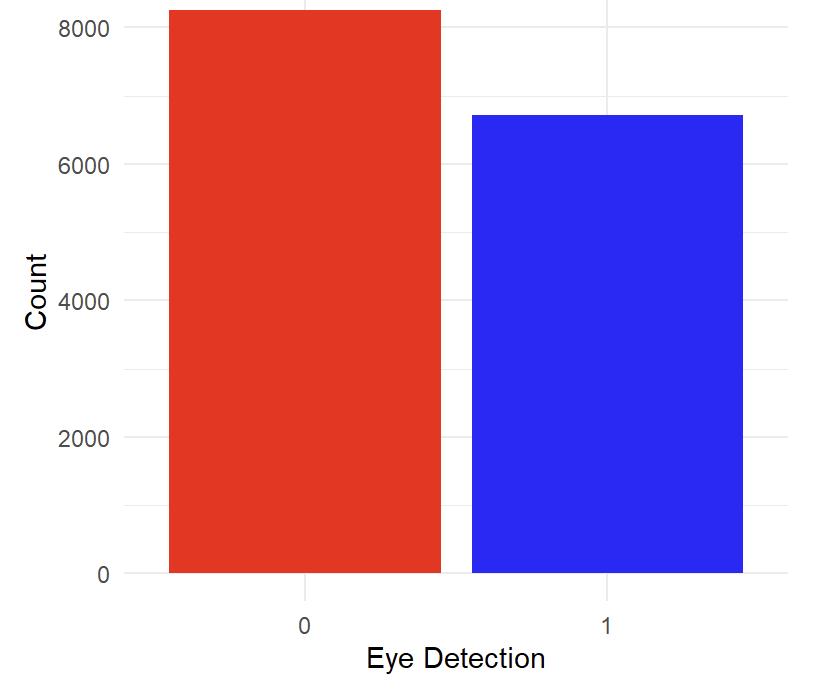
\includegraphics[width=0.4\linewidth]{figure/3} 

}

\caption{Distribution of Eye Detection (Target variable)}\label{fig:unnamed-chunk-1}
\end{figure}

\subsection{4.2.2 Correlation}\label{correlation}

\textbf{Figure 2} shows the degree of signal synchrony across different brain regions. Overall, most of the correlations are positive, particularly between spatially adjacent or functionally related regions such as O2 and T8 (r = 0.87) and AF3 and AF4 (r = 0.96), indicating highly synchronized neural activity during the recording period. However, some inter-regional pairs show notably lower correlations, such as F7 and AF4 (r = 0.14) or F7 and FC5 (r = 0.05), suggesting more independent or unsynchronized neural activities between these areas.

\begin{figure}[H]

{\centering 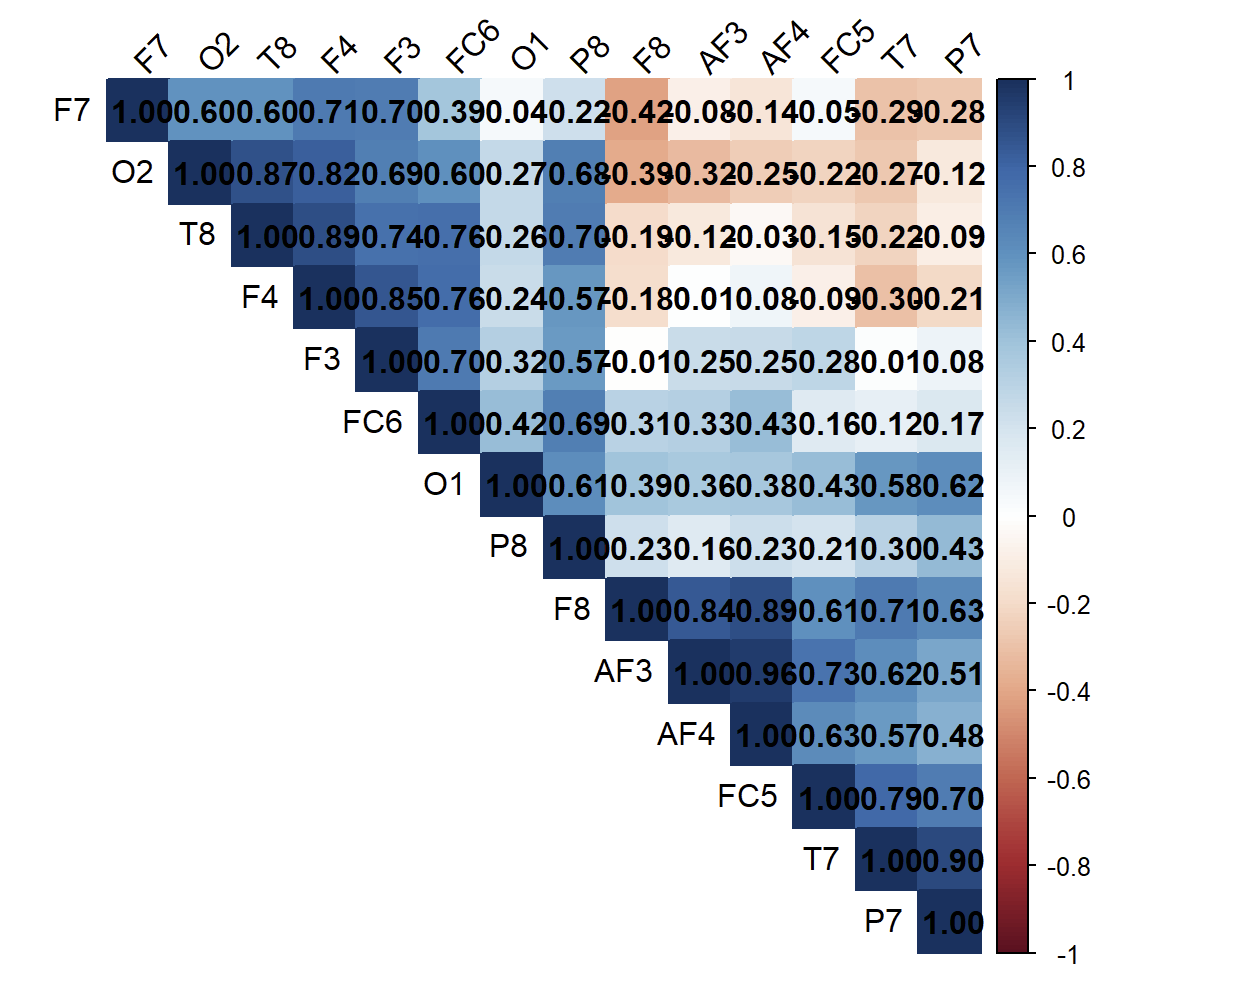
\includegraphics[width=0.8\linewidth]{figure/2} 

}

\caption{Pearson correlation coefficient heatmap}\label{fig:unnamed-chunk-2}
\end{figure}

\newpage

\subsection{4.2 Feature selection}\label{feature-selection}

\textbf{Figure 3} shows that 57 features with non-zero coefficients are selected by LASSO, covering original EEG channels, frequency domain features, and interaction features. In detail, fft\_theta\_power\_f4 (coefficient is 0.630) showed the largest positive effect, indicating that the power of the theta frequency band (4--8 Hz) in the prefrontal region (F4) plays an important role in eye state classification. Similarly, fft\_beta\_power\_p7 (coefficient is 0.517) and fft\_beta\_power\_f7 (coefficient is 0.476) also show large positive contributions, indicating that activities in the Beta band (13--30 Hz) in the occipital lobe (P7) and prefrontal lobe (F7) are closely related to the eye state. In contrast, fft\_beta\_power\_p8 (coefficient is −0.541) and f7 (coefficient is −0.726) showed large negative effects, indicating that increases in these features may affect the eyes closed condition.

\begin{figure}[H]

{\centering 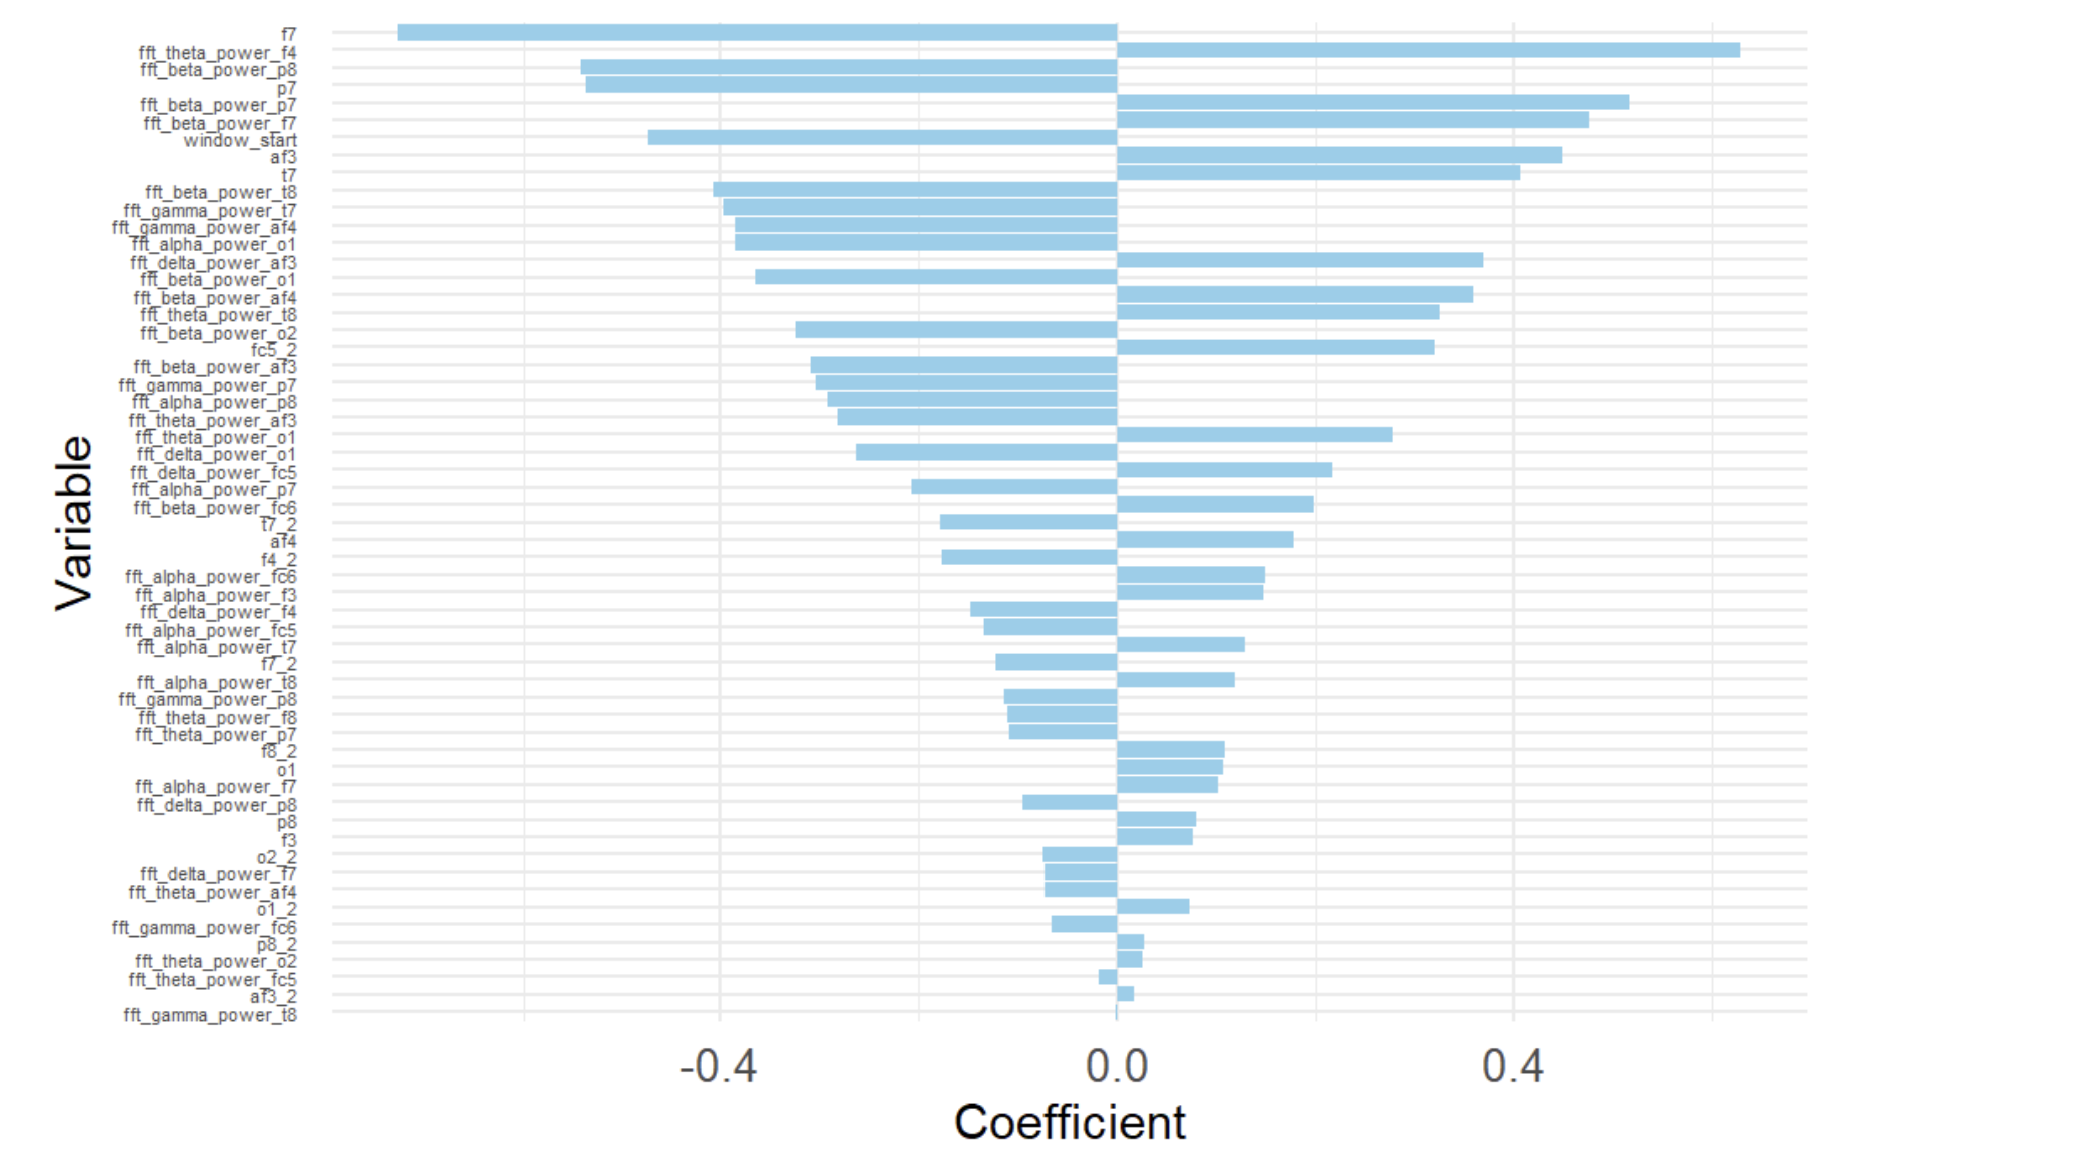
\includegraphics[width=1.2\linewidth]{figure/4} 

}

\caption{LASSO Selected Variables Coefficients}\label{fig:unnamed-chunk-3}
\end{figure}

Random forest analysis further ranked the feature importance and select the top 30 features for model training (\textbf{Table 3}). \textbf{Figure 4} shows the importance of the top 10 features. In detail, \texttt{window\_start} (importance 42.81) shows the highest contribution, indicating that the starting point of the time window plays a significant role in classification. Frequency domain features such as \texttt{fft\_beta\_power\_p8} (importance 13.94), \texttt{fft\_delta\_power\_o1} (importance 8.22), and \texttt{fft\_beta\_power\_o1} (importance 8.12) ranked at the top, indicating that the power of Beta band (13--30 Hz) and Delta band (0.5--4 Hz) in the occipital (\texttt{P8}, \texttt{O1}) and prefrontal (\texttt{AF3}) regions are crucial for eye state prediction. Raw EEG channels such as \texttt{p7} (importance 7.04) and \texttt{o1} (importance 6.18) also show some importance. The selection of these features will effectively reduce redundancy and collinearity, providing a robust foundation for subsequent modeling.

\begin{table}[!h]
\centering
\caption{\label{tab:unnamed-chunk-4}Variable Importance for EEG Features}
\centering
\begin{tabular}[t]{l|r|l|r}
\hline
Variable & Importance & Variable & Importance\\
\hline
window\_start & 42.806 & fft\_gamma\_power\_t7 & 3.564\\
\hline
fft\_beta\_power\_p8 & 13.937 & f7 & 3.471\\
\hline
fft\_delta\_power\_o1 & 8.218 & fft\_beta\_power\_af3 & 3.453\\
\hline
fft\_beta\_power\_o1 & 8.122 & fft\_gamma\_power\_p7 & 3.307\\
\hline
fft\_gamma\_power\_p8 & 7.762 & fft\_delta\_power\_p8 & 3.143\\
\hline
p7 & 7.040 & fft\_theta\_power\_f4 & 3.016\\
\hline
fft\_theta\_power\_o1 & 6.701 & p8 & 2.972\\
\hline
o1 & 6.182 & fft\_theta\_power\_p7 & 2.894\\
\hline
af4 & 5.947 & fft\_alpha\_power\_t7 & 2.729\\
\hline
af3 & 5.644 & o1\_2 & 2.675\\
\hline
fft\_alpha\_power\_p7 & 5.304 & fft\_alpha\_power\_t8 & 2.633\\
\hline
fft\_beta\_power\_t8 & 4.271 & f3 & 2.497\\
\hline
fft\_beta\_power\_o2 & 3.789 & fft\_alpha\_power\_fc6 & 2.494\\
\hline
fft\_alpha\_power\_p8 & 3.617 & fft\_delta\_power\_f4 & 2.469\\
\hline
fft\_alpha\_power\_o1 & 3.567 & fft\_alpha\_power\_f3 & 2.462\\
\hline
\end{tabular}
\end{table}

\begin{figure}[H]

{\centering 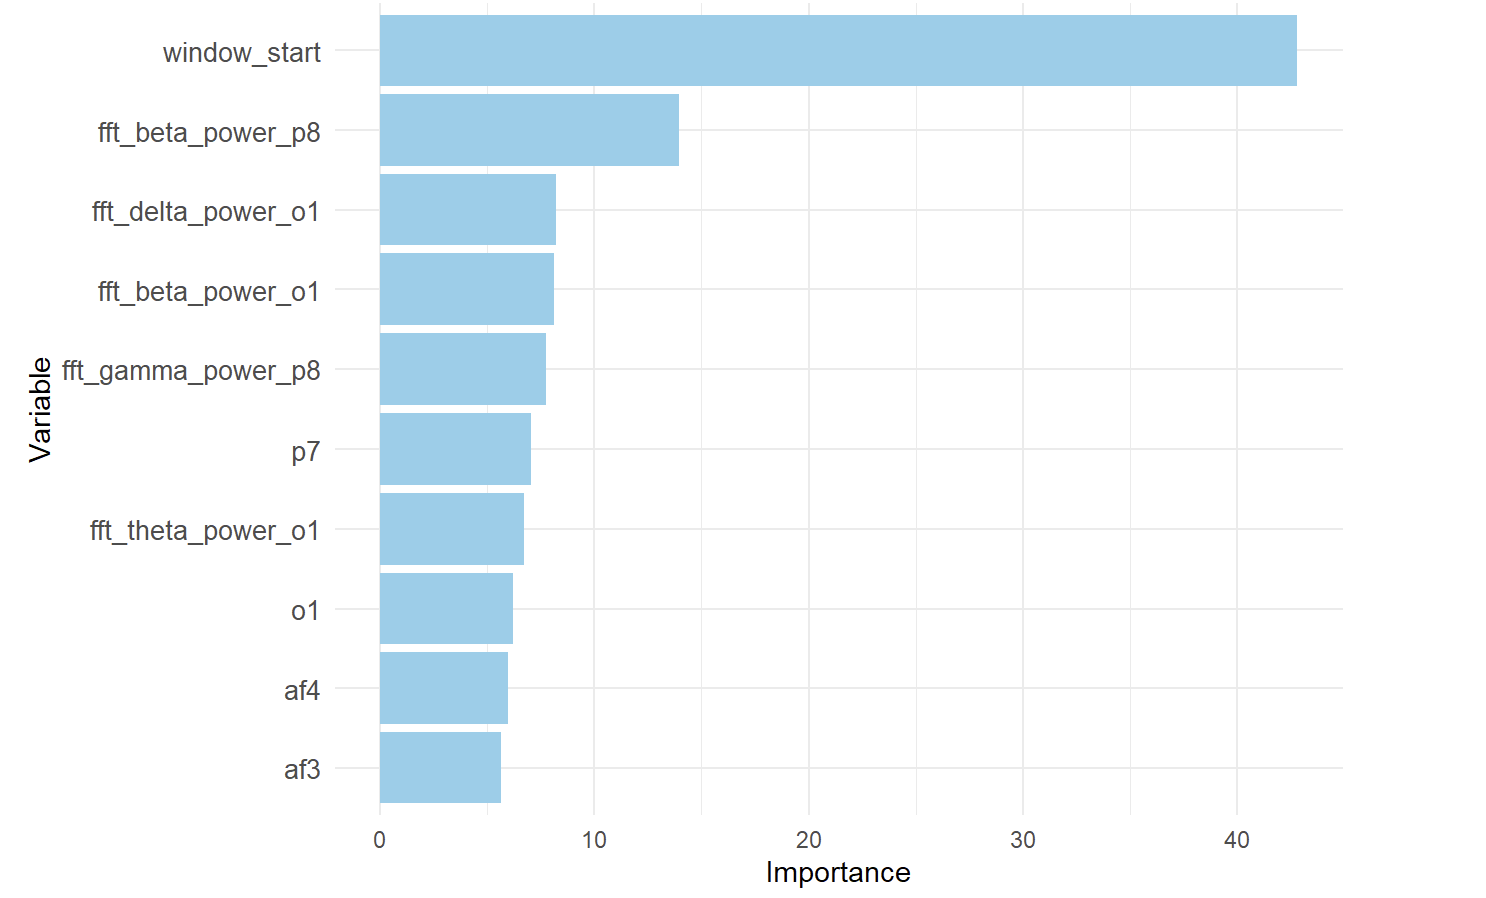
\includegraphics[width=0.8\linewidth]{figure/5} 

}

\caption{Top 10 Variables Importance}\label{fig:unnamed-chunk-5}
\end{figure}

\newpage

\subsection{4.3 Model performance}\label{model-performance}

\textbf{Table 4} summarizes the evaluation metrics of the five models (random forest, logistic regression, SVM, MLP, and kNN). Random forest is used as the baseline model for feature selection, with an accuracy of 0.989 and 0.917 on the training and testing sets, respectively, and the AUC value is 0.974, showing excellent discrimination ability but a certain risk of overfitting. Logistic regression was trained using 30 features selected by random forest, with a training accuracy of 0.757, a testing accuracy of 0.750, and an AUC value of 0.822, which is much worse. The SVM model achieved an accuracy of 0.989 and 0.946 on the training and testing sets, respectively, and the AUC value is 0.982, showing the best discrimination ability. The training set accuracy of the MLP model is 0.994, the test set accuracy is 0.922, and the AUC value is 0.958, the testing performance is only worse than SVM. The kNN model has a training set accuracy of 0.973, a test set accuracy of 0.917, and an AUC value of 0.982, which is slightly lower than SVM and MLP, but still better than logistic regression.

\begin{table}[!h]
\centering
\caption{\label{tab:unnamed-chunk-6}Comparison of Model Performance Metrics}
\centering
\begin{tabular}[t]{l|r|r|r|r|r|r}
\hline
Model & Train\_Accuracy & Test\_Accuracy & AUC & Precision & Recall & F1\_Score\\
\hline
Random Forest & 0.989 & 0.917 & 0.974 & 0.897 & 0.941 & 0.919\\
\hline
Logistic Regression & 0.757 & 0.750 & 0.822 & 0.774 & 0.706 & 0.738\\
\hline
SVM & 0.989 & 0.946 & 0.982 & 0.917 & 0.980 & 0.948\\
\hline
MLP & 0.994 & 0.922 & 0.958 & 0.913 & 0.931 & 0.922\\
\hline
kNN & 0.973 & 0.917 & 0.982 & 0.947 & 0.882 & 0.914\\
\hline
\end{tabular}
\end{table}

\textbf{Figure 5} shows the ROC curves of the five models. The ROC curves of SVM and kNN are closest to the upper left corner, with AUC values of 0.982, respectively, showing the highest discrimination ability, followed by random forest (AUC = 0.974) and MLP (AUC = 0.958), while logistic regression has the lowest AUC value (0.822), showing the worst discrimination ability.

\begin{figure}[H]

{\centering 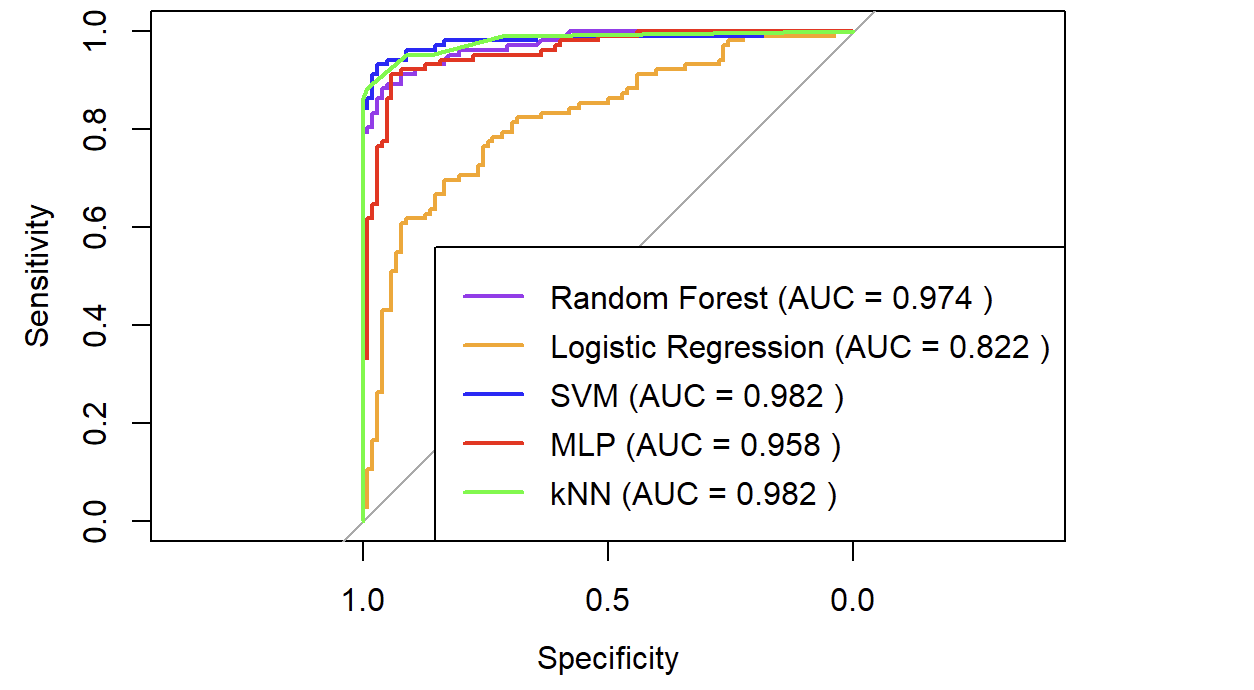
\includegraphics[width=0.85\linewidth]{figure/6} 

}

\caption{ROC Curves for All Models}\label{fig:unnamed-chunk-7}
\end{figure}

\newpage

\textbf{Table 5} shows the results of the McNemar test. There was a significant difference in the prediction performance between logistic regression and other models (p \textless{} 0.001), indicating that the error pattern of logistic regression was different from that of other models and its overall performance was poor. This is consistent with its lower test accuracy (0.750) and AUC value (0.822). There were no significant differences in the prediction performance between random forest, SVM, MLP, and kNN (p-values ranged from 0.211 to 1), indicating that the error patterns of these models were highly consistent. Among them, the p-value of SVM and MLP is 0.332, the p-value of SVM and kNN is 0.211, while the p-values of random forest and MLP, random forest and kNN, and MLP and kNN are all 1, indicating that the prediction behaviors of these models on the test data are very similar.

\begin{table}[!h]
\centering
\caption{\label{tab:unnamed-chunk-8}McNemar's Test p-values for Pairwise Model Comparisons}
\centering
\begin{tabular}[t]{l|r}
\hline
Comparison & p.value\\
\hline
Random Forest vs Logistic Regression & 0.0000004\\
\hline
Random Forest vs SVM & 0.3319755\\
\hline
Random Forest vs MLP & 1.0000000\\
\hline
Random Forest vs kNN & 1.0000000\\
\hline
Logistic Regression vs SVM & 0.0000000\\
\hline
Logistic Regression vs MLP & 0.0000002\\
\hline
Logistic Regression vs kNN & 0.0000031\\
\hline
SVM vs MLP & 0.3319755\\
\hline
SVM vs kNN & 0.2112995\\
\hline
MLP vs kNN & 1.0000000\\
\hline
\end{tabular}
\end{table}

\subsection{4.4 Learning Curve}\label{learning-curve}

\textbf{Figure 6} shows the learning curves of five models (random forest, logistic regression, SVM, MLP, and kNN), depicting the effect of training sample size on training accuracy and test accuracy. The training accuracy of the random forest (purple line) climbs steadily from 0.95 to nearly 1.0, but the test accuracy stabilizes between about 0.9 and 0.92, showing some tendency to overfit, especially when the training sample size is small (200 to 400). This is consistent with the phenomenon that its training set accuracy (0.989) is much higher than the test set accuracy (0.917). It may be that the sample repetition caused by oversampling enhances the model's ability to fit the training data. The training and test accuracies of logistic regression (orange line) are both low, around 0.70 to 0.80, indicating that its model is unable to fully utilize the characteristics of the data for prediction, which is consistent with its low test accuracy (0.750) and AUC value (0.822).

The training accuracy of SVM (blue line) is close to 1.0, and the test accuracy gradually increases from 0.83 to about 0.95, and tends to stabilize when the sample size reaches 500, showing good generalization ability. This is consistent with its test set accuracy (0.946) and AUC value (0.982), demonstrating the robustness of SVM in high-dimensional feature space. The training accuracy of MLP (red line) reaches up to 0.994, and the test accuracy increases from 0.78 to 0.92 and remains stable when the sample size increases, indicating that its nonlinear modeling ability effectively captures the complex patterns of EEG signals. The training and test accuracy of kNN (green line) improves with the increase of sample size, with the test accuracy rising from 0.80 to 0.92, and approaching the performance of SVM and MLP.

Overall, the learning curves of SVM, MLP, and kNN show good generalization ability, and the test accuracy tends to converge when the sample size reaches 500, while the overfitting risk of random forest and the low performance of logistic regression show that these two models are not applicable. This result is consistent with the conclusion of the McNemar test, where there was no significant difference in the prediction performance of random forest, SVM, MLP, and kNN (p-values ranged from 0.211 to 1), while logistic regression was significantly inferior to the other models (p-values \textless{} 0.001).

\begin{figure}[H]

{\centering 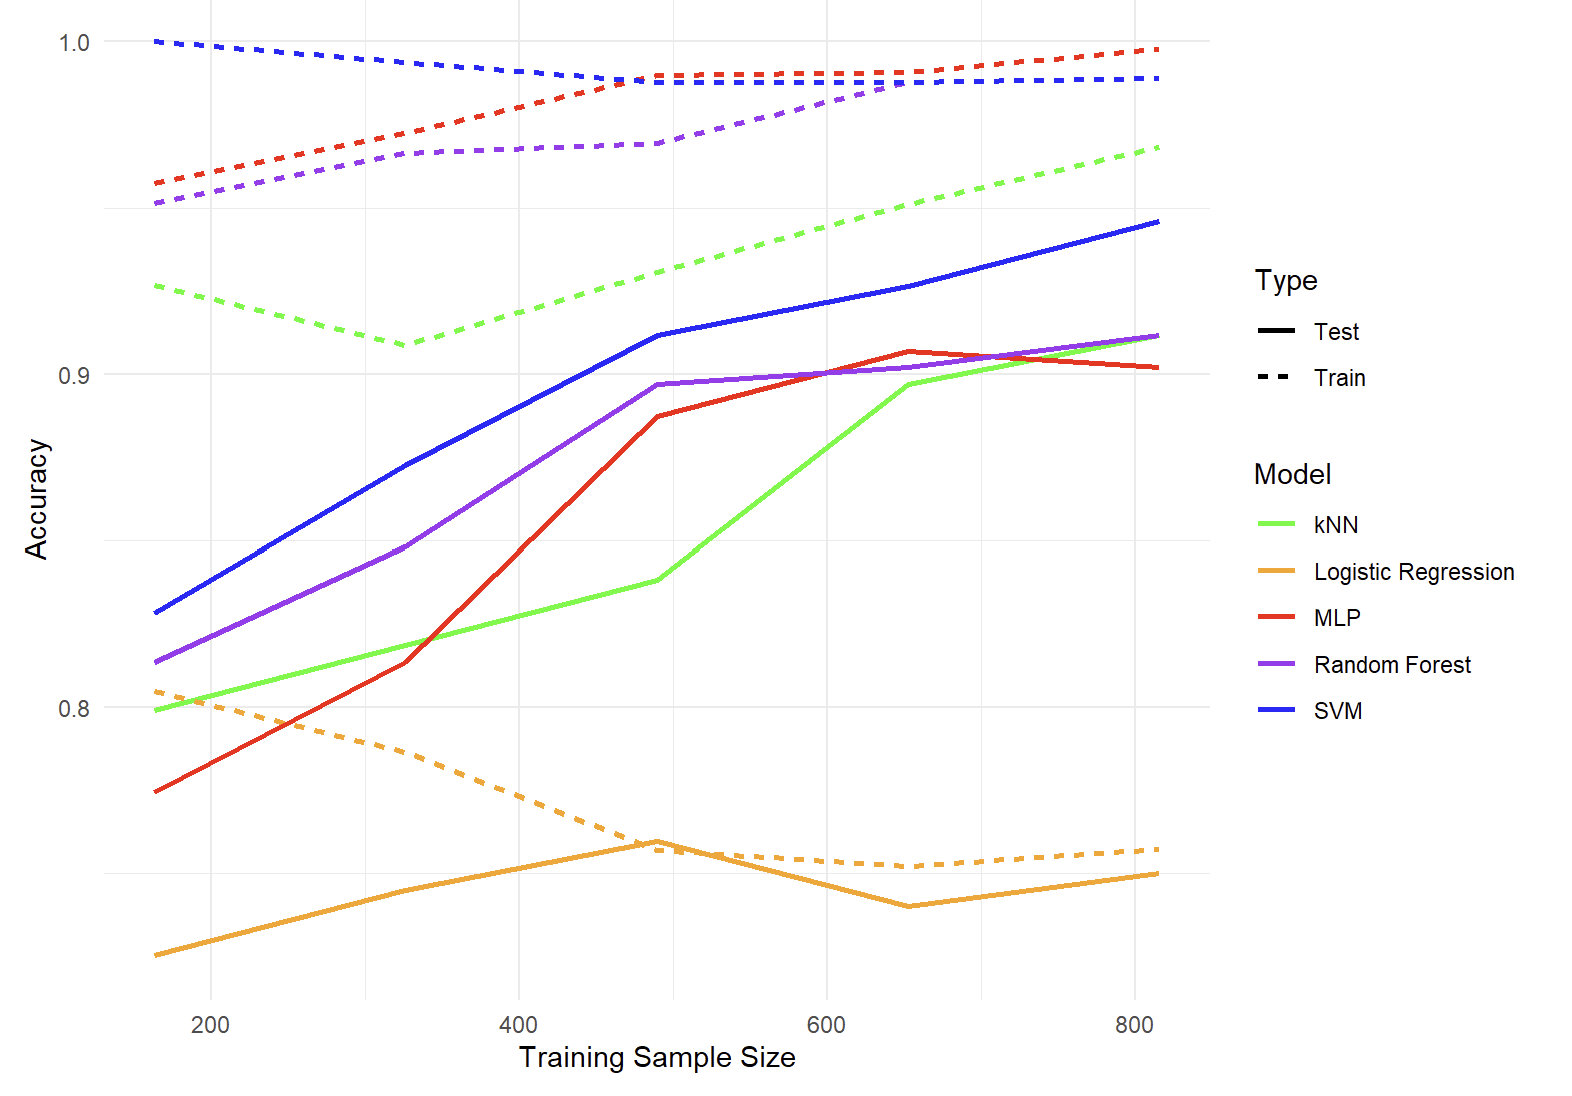
\includegraphics[width=0.85\linewidth]{figure/7} 

}

\caption{Learning Curves for All Models}\label{fig:unnamed-chunk-9}
\end{figure}

\section{V. Conclusion and Future Work}\label{v.-conclusion-and-future-work}

\subsection{5.1 Conclusion}\label{conclusion}

This study successfully achieved eye state classification using EEG signal datasets by combining feature engineering, LASSO and random forest for feature selection and applying five machine learning models. The top 30 important features selected by LASSO and random forest (especially \texttt{window\_start} and Beta and Delta band features) provide a robust prediction basis for subsequent model training. The SVM model performed best among all models, with a test set accuracy of 0.946 and an AUC value of 0.982. By adding reasonable interaction features through domain knowledge, the model can further capture the joint effects or coordinated change patterns between different brain regions and thus improve classification efficiency. Feature engineering and data balancing strategies have significantly improved model performance. The results of this study once again demonstrated the capabilities of machine learning technology in EEG classification tasks, and also provided reliable technical support for applications such as driving fatigue monitoring and attention assessment.

\subsection{5.2 Future work}\label{future-work}

Future research can be extended in several directions. First, we can try to introduce more expressive deep learning models, such as convolutional neural networks (CNNs) and long short-term memory networks (LSTMs), to automatically learn spatial and temporal features from raw EEG time series data and reduce reliance on manual feature engineering. Secondly, in order to improve the interpretability of the model, methods such as layer-wise relevance propagation (LRP) or attention mechanism can be applied to help analyze the brain areas and frequency bands that the model focuses on during classification, thereby improving the credibility of the model in clinical applications. In addition, although the existing oversampling method can balance the data, it may also cause overfitting problems. Therefore, it is recommended to explore more advanced sample synthesis techniques in the future, such as SMOTE or ADASYN, to improve the generalization ability of the model. Finally, we can further collect EEG data from subjects of different age groups and conditions to establish a more representative and externally valid dataset, and integrate other physiological signals (such as eye movements or electrocardiograms) for multimodal analysis to improve classification accuracy and expand its application potential in areas such as attention monitoring, driving safety, and medical auxiliary diagnosis.

\newpage

\section{VI. References}\label{vi.-references}

\phantomsection\label{refs}
\begin{CSLReferences}{1}{0}
\bibitem[\citeproctext]{ref-ma2020eeg}
Ma, J., \& Gao, L. (2020). EEG-based eye state prediction using feature interactions and LSTM networks. \emph{IEEE Access}, \emph{8}, 163651--163659. \url{https://doi.org/10.1109/ACCESS.2020.3022061}

\bibitem[\citeproctext]{ref-roesler2013eyestate}
Roesler, O., \& Suendermann, D. (2013). A first step towards eye state prediction using EEG. \emph{International Conference on Applied Informatics for Health and Life Sciences}. Istanbul, Turkey. Retrieved from \url{http://ehrai.com/su/pdf/aihls2013.pdf}

\bibitem[\citeproctext]{ref-sabanci2015classification}
Sabanci, K., \& Koklu, M. (2015). The classification of eye state by using kNN and MLP classification models according to the EEG signals. \emph{International Journal of Intelligent Systems and Applications in Engineering}, \emph{3}(4), 127--130.

\bibitem[\citeproctext]{ref-singla2011comparison}
Singla, R., Singh, A., \& Jha, S. (2011). Comparison of SVM and ANN for classification of eye events in EEG. \emph{Journal of Biomedical Science and Engineering}, \emph{4}(1), 62--69. \url{https://doi.org/10.4236/jbise.2011.41008}

\bibitem[\citeproctext]{ref-uci_eeg_eyestate}
UCI Machine Learning Repository. (2013). \emph{EEG eye state}. UCI Machine Learning Repository. Retrieved from \url{https://archive.ics.uci.edu/dataset/264/eeg+eye+state}

\bibitem[\citeproctext]{ref-wang2014eye}
Wang, Y., Chen, X., \& Zhang, Y. (2014). Eye state recognition from EEG data using incremental attribute learning. \emph{Computational and Mathematical Methods in Medicine}, \emph{2014}, 1--10. \url{https://doi.org/10.1155/2014/365101}

\end{CSLReferences}


\end{document}
